\chapter{Permutations, Cosets, and Direct Products}

\section{Groups of Permutations}

\begin{definition}[Permutation of a set]
    A \emph{permutation of a set} $A$ is a function $\phi\colon A \to A$ that is both one to one and onto.
\end{definition}
\begin{remark}[Permutation Multiplication]
    Function composition $\circ$ is a binary operation on the collection of all permutations of a set $A$. We call this operation \emph{permutation multiplication}.
\end{remark}
\begin{remark}
    Let $\sigma, \tau$ be permutations of a set $A$ so $\sigma, \tau$ are both one-to-one function mapping $A$ onto $A$. then, $\sigma\circ\tau$, or simply $\sigma\tau$ is a permutation as long as it is one-to-one.

    For any $a_1,a_2 \in A$, if $(\sigma\tau)(a_1)=(\sigma\tau)(a_2)$ gives $(\sigma(\tau(a_1)))=(\sigma()\tau(a_1))$. Because $\sigma$ is injective, $\tau(a_1)=\tau(a_2)$. Because $\tau$ is injective, $a_1=a_2$ so $\sigma\tau$ is injective.

    For any $a \in A$, there exists some $b in A$ so $\sigma(b) = a$ because $\sigma$ is onto $A$. Because $\tau$ is onto $A$, there exists some $c \in A$ so $\tau(c) = b$. Thus, $a = (\sigma\tau)(c)$ so $\sigma\tau$ is onto $A$.
\end{remark}
\begin{example}
    Given a set $A = \{1,2,3,4,5\}$, we can write a permutation $\sigma$ as 
    \[\sigma =
    \begin{pmatrix}
        1 & 2 & 3 & 4 & 5 \\
        4 & 2 & 5 & 3 & 1
    \end{pmatrix}.\] so $\sigma(1) = 4$, etc.
\end{example}
\begin{theorem}
    Let $A$ be a nonempty set, and $S_A$ be the collection of all permutations of $A$. Then, $S_A$ is a group under permutation multiplication.
\end{theorem}
\begin{proof}
    Because the composition of two permutations of $A$ results in a permutation, we have closure under $\circ$. For any functions $f,g,h$, $((f\circ g)\circ h)(x) = (f(g))\circ(h)(x) = f(g(h))(x) = f(g\circ h)(x)$ so $\mathscr{G}_1$ is easily satisfied. The permutation $\imath$ defined as $\imath(a)=a$ for all $a \in A$ is the identity ($\mathscr{G}_2$). Last, for any permutation $\sigma$, $\sigma^{-1}$ reverse the direction of the mapping $\sigma$ such that $\sigma^{-1}(a)$ is the element $a'$ of $A$ so $\sigma(a')=a$. This exists because $\sigma$ is bijective. For any $a \in A$, $\imath(a) = a = \sigma(a') = \sigma(\sigma^{-1}(a')) = (\sigma\sigma^{-1})(a)$ and $\imath(a') = a' = \sigma^{-1}(a) = \sigma^{-1}(\sigma(a')) = (\sigma^{-1}\sigma)(a')$ satisfying $\mathscr{G}_3.$
\end{proof}
\begin{remark}
    To define an isomorphism $\phi\colon S_A \to S_B$, we let $f \colon A \to B$ have one-to-one function mapping $A$ onto $B$ so $A$ and $B$ have the same cardinality so for $\sigma \in S_A$, let $\phi(\sigma) = \bar{\sigma}\in S_B$ so that for all $a \in A$, $\bar{\sigma}(f(a)) = f(\sigma(a)).$ 
\end{remark}
\begin{definition}[Symmetric Group on $n$ Letters]
    Let $A$ be the finite set $\{1,2,\dots,n\}$. The group of all permutations of $A$ is the \emph{symmetric group on $n$ letters} $S_n$. Note that $S_n$ has $n!$ elements.
\end{definition}
\begin{remark}
    $S_3$ is also the 3rd dihedral group $D_3$ of \emph{symmetries of an equilateral triangle} where $\rho_i$ is rotations and $\mu_i$ is mirror images in bisectors of angles such that $D_3$ is made up of:
    \[
    \begin{Bmatrix}
        \rho_0 = \begin{pmatrix} 1 & 2 & 3 \\ 1 & 2 & 3 \end{pmatrix}, &
        \mu_0 = \begin{pmatrix} 1 & 2 & 3 \\ 1 & 3 & 2 \end{pmatrix}, \\
        \rho_1 = \begin{pmatrix} 1 & 2 & 3 \\ 2 & 3 & 1 \end{pmatrix}, &
        \mu_1 = \begin{pmatrix} 1 & 2 & 3 \\ 3 & 2 & 1 \end{pmatrix}, \\
        \rho_2 = \begin{pmatrix} 1 & 2 & 3 \\ 3 & 1 & 2 \end{pmatrix}, &
        \mu_2 = \begin{pmatrix} 1 & 2 & 3 \\ 2 & 1 & 3 \end{pmatrix}.        
    \end{Bmatrix}
    \]
\end{remark}
\begin{definition}[$n$th Dihedral Group $D_n$]
    The \emph{$n$th dihedral group $D_n$} is the group of symmetries of the regular $n$-gon.
\end{definition}
\begin{example}[Octic Group $D_4$]
    Given a square: 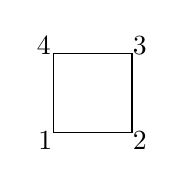
\begin{tikzpicture}
        \draw (0cm,0cm) rectangle (1cm, 1cm);
        \foreach \x/\y/\n in {-.1/-.1/1, 1.1/-.1/2, 1.1/1.1/3, -.12/1.1/4}{\node at (\x cm, \y cm) {\n};}\end{tikzpicture}
    , $D_4$ is the set of:
    \[
        \begin{Bmatrix}
            \rho_0 = \begin{pmatrix} 1 & 2 & 3 & 4\\ 1 & 2 & 3 & 4 \end{pmatrix}, &
            \mu_0 = \begin{pmatrix} 1 & 2 & 3 & 4 \\ 2 & 1 & 4 & 3 \end{pmatrix}, \\
            \rho_1 = \begin{pmatrix} 1 & 2 & 3 & 4\\ 2 & 3 & 4 & 1 \end{pmatrix}, &
            \mu_1 = \begin{pmatrix} 1 & 2 & 3 & 4 \\ 4 & 3 & 2 & 1 \end{pmatrix}, \\
            \rho_2 = \begin{pmatrix} 1 & 2 & 3 & 4\\ 3 & 4 & 1 & 2 \end{pmatrix}, &
            \delta_0 = \begin{pmatrix} 1 & 2 & 3 & 4 \\ 3 & 2 & 1 & 4 \end{pmatrix}, \\
            \rho_3 = \begin{pmatrix} 1 & 2 & 3 & 4\\ 4 & 1 & 2 & 3 \end{pmatrix}, &
            \delta_1 = \begin{pmatrix} 1 & 2 & 3 & 4 \\ 1 & 4 & 3 & 2 \end{pmatrix}.
        \end{Bmatrix}
        \]
    where $\rho_i, \mu_i, \delta_i$ represent rotations, mirror images in perpendicular bisectors of sides, and diagonal flips respectively.
\end{example}
\begin{definition}[Image of $H$ under $f$]
    Let $f\colon A\to B$ be a function and $H$ be a subset of $A$. The \emph{image of $H$ under $f$} is the set $\{f(h) \mid h \in H\}$ and is denoted $f[H].$
\end{definition}
\begin{lemma}
    Let $G, G'$ be groups and $\phi\colon G\to G'$ be a one-to-one function such that for all $x,y \in G$, $\phi(xy) = \phi(x)\phi(y).$ Thus $\phi[G]$ is a subgroup of $G'$ and $\phi$ provides an isomorphism of $G$ with $\phi[G]$.
\end{lemma}
\begin{proof}
    We simply prove the subgroup requirements. For any $x', y' \in \phi[G]$, there exist $x,y \in G$ so $\phi(x)=x'$ and $\phi(y)=y'$. By hypothesis, $\phi(xy) = \phi(x)\phi(y)$ so $x'y' \in \phi[G]$ so $\phi[G]$ is closed under the operation of $G'$. Next, say $e'$ is the identity of $G'$. Then, $e'\phi(e) = \phi(e) = \phi(ee) = \phi(e)\phi(e)$. Cancellation in $G'$ shows $e'=\phi(e)$ so $e' \in \phi[G]$. Last, for any $x' \in \phi[G]$, $e'=\phi(e)=\phi(xx^{-1})=\phi(x)\phi(x^{-1})=x'\phi(x^{-1})$ implying $x'^{-1} = \phi(x^{-1}) \in \phi[G]$. Thus $\phi[G]$ is a subgroup of $G'$. We already showed $\phi$ is onto and therefore an isomorphism of $G$ with $\phi[G]$.
\end{proof}
\begin{theorem}[Cayley's Theorem]
    Every group is isomorphic to a group of permutations.
\end{theorem}
\begin{proof}
    Let $G$ be a group. We want to show $G$ is isomorphic to a subgroup of $S_G$. By the previous lemma, we need only define a universal one-to-one function $\phi\colon G\to S_G$ with the homomorphism property. For any $x,g \in G$, let's define left multiplication by x via $\lambda_x\colon G\to G$ as $\lambda_x(g)=xg$. For all $c \in G$, $\lambda_x(x^-1c)=x(x^-1c)=c$ so clearly $\lambda_x$ maps $G$ onto $G$. Also, for any $a,b \in G$, $\lambda_x(a)=\lambda_x(b) \implies xa=xb \implies a=b$ through left cancellation. Thus, $\lambda_x$ is one-to-one, onto, and a permutation of $G$. Now, we define $\phi\colon G\to S_G$ as $\phi(x)=\lambda_x$ for all $x\in G$.

    To satisfy our lemma, we now only show $\phi$ is one-to-one and has the homomorphism property. Let $e$ be the identity on $G$ so that $\phi(x)=\phi(y)$ implies $\lambda_x=\lambda_y$ so $\lambda_x(e)=\lambda_y(e)\implies xe=ye \implies x=y$. Last, for any $x,y,g\in G$, $\lambda_{xy}(g) = (xy)g = x(yg) = \lambda_x(\lambda_y(g)) = \lambda_x\lambda_y(g)$ so $\phi(xy)=\phi(x)\phi(y)$ satisfying the homomorphism property.
\end{proof}
\begin{definition}[Left/Right Regular Representation]
    The map $\phi\colon G \to S_G$ defined as above is the \emph{left regular represention} of $G$ and the map $\mu\colon G \to S_G$ defined by $\mu(x)=\rho_{x^{-1}}$ where $\rho_x(g)=gx$ for all $x,g\in G$ is the \emph{right regular representation} of $G$.
\end{definition}

\section{Orbits, Cycles, and the Alternating Groups}

\begin{definition}[Orbit of $a$ under $\sigma \in S_A$]
    Let $A$ be a set and $\sigma \in S_A$. For a fixed $a \in A$, the set $\mathcal{O}_{a.\sigma}=\{\sigma^n(a)\mid n\in\Z\}$ is the \emph{orbit of $a$ under $\sigma$.}
\end{definition}
\begin{remark}
    Let $\sigma$ be a permutation of a set $A$. The equivalence classes in $A$ are determined by the following equivalence class:
    \begin{center}
        For $a,b \in A$, let $a\sim b$ if and only if $b = \sigma^n(a)$ for some $n \in \Z$.
    \end{center}
    These are called the \emph{orbits of $\sigma$}.
\end{remark}
\begin{explanation}
    $\sim$ is an equivalence relation because it is:
    \begin{enumerate}
        \item \textbf{reflexive:} $a\sim a$ clearly because $a=\imath(a)=\sigma^0(a)$.
        \item \textbf{symmetric:} If $a \sim b$, then $b = \sigma^n(a)$ for some $n \in \Z$ so $a = \sigma^{-n}(b)$ and $-n \in \Z$ so $b\sim a$.
        \item \textbf{transitive:} If $a \sim b, b \sim c$, then $b = \sigma^n(a)$ and $c = \sigma^m(b)$ for some $n,m \in \Z$. This implies $c = \sigma^m(\sigma^n(a)) = \sigma^{n+m}(a)$ so $a \sim c$.
    \end{enumerate}
\end{explanation}
\begin{example}
    The orbits of $\imath$ are the singleton subsets of $A$.
\end{example}
\begin{example}
    Given the permutation $\sigma$ of a finite set $A$ defined as:
    \[\sigma = \begin{pmatrix}
        1 & 2 & 3 & 4 & 5 & 6 & 7 & 8 \\ 3 & 8 & 6 & 7 & 4 & 1 & 5 & 2
    \end{pmatrix},\]
    we can map each cycle in the following ways:
    \begin{center}
        \begin{tikzpicture}
            \node [circle, draw, minimum size = 2cm, postaction={decorate}, decoration={markings, mark=between positions .083 and 1.000 step 0.333 with {\arrow{>}}}] (1) at (0,0) {};
            \node [circle, draw, minimum size = 2cm, postaction={decorate}, decoration={markings, mark=between positions .500 and 1.000 step 0.500 with {\arrow{>}}}] (2) at (3cm, 0) {};
            \node [circle, draw, minimum size = 2cm, postaction={decorate}, decoration={markings, mark=between positions .083 and 1.000 step 0.333 with {\arrow{>}}}] (3) at (6cm, 0) {};

            \foreach \n/\circ/\rad\direc in {1/1/-.083/right, 3/1/.250/above, 6/1/.583/left, 2/2/.250/above, 8/2/.750/below, 4/3/.250/above, 7/3/.583/left, 5/3/.916/right}
            {
                \node[draw, thick, fill, inner sep = .3mm, circle, label = \direc:\n] at (\circ.\rad*360) {};
            }

            % \draw (\a*360/17: 4cm) node{angle \a};
        \end{tikzpicture}
    \end{center}
\end{example}


section 9.

% \section{Cosets and the Theorem of Lagrange}

% \section{Direct Products and Finitely Generated Abelian Groups}

% \section{Plane Isometries}